\documentclass[hyperref={pdfpagelabels=false}]{beamer}
\setbeamercolor{background canvas}{bg=white}
\usepackage{graphicx,lmodern,subfigure,ulem,color,graphicx,tikz,booktabs,natbib}
\usepackage{mathrsfs}
\usetheme{Warsaw}
%\definecolor{beamer@blendedblue}{rgb}{0.1,0.5,0.1}
%\definecolor{ForestGreen}{RGB}{60, 140, 60}
%\setbeamercolor{structure}{fg=beamer@blendedblue}
\setbeamertemplate{navigation symbols}{}
\setbeamertemplate{footline}[frame number]
\bibliographystyle{chicago}
\newcommand{\spitem}{\vspace{.3cm}\item}
\newcommand{\elas}{$E_{labor}$}
%\def \FigPath {Users\th3\Documents\Job_Market_Paper\Code\Figures} 
\DeclareMathOperator{\E}{\mathbb{E}}
\usepackage{makecell}




\title{Financial and Uncertainty Shocks}
\author{Marco Brianti}
\institute{Boston College}
\date{October 2018}

\usetheme[
outer/progressbar=foot,
outer/numbering=none
]{metropolis}


\begin{document}
	
	\frame{\titlepage \begin{center} Dissertation Project \end{center} }
	

	
	
		\frame{\frametitle{Alternative Drivers of Economic Fluctuations}
			
			\	
			
			\textit{The shocks that produced the recession were primarily associated with \textbf{financial disruptions} and \textbf{heightened uncertainty}}
			
			\hfill  Stock and Watson (2012) 
			%Stock and Watson (2012) comprehensive empirical anatomy of the Great recession
			%The shocks that produced the recession were primarily associated with financial disruptions and heightened uncertainty		
			
			
			\
			

			
Depth and duration of \textbf{financial crisis} 
\begin{itemize}
	\item[$\Rightarrow$] several challenges for standard business cycle models
\end{itemize}  
% who used traditional sources of BC fluctuations such as productivity shocks. In particular, those models together with those shocks were unable to explain important features specifically related to the financial crisis.

\

%In response to this limitation,		
New strands of literature arose proposing alternative shocks
\begin{enumerate}
	\item \textbf{Financial shocks} - Khan and Thomas (2013) JPE %among others Jerman and Quadrini (2012) AER, Christiano, Motto e Rostagno (2010) Working paper
	\item \textbf{Uncertainty shocks} - Bloom (2009) ECMA %was the first to estimate the dynamic effect of uncertainty in a both an empirical and theoretical context 
	\end{enumerate}

\




	}

	\frame{\frametitle{Theoretical Definitions}	
		
%Important to define because both shocks are residuals from endogenouse proxy variables that depends on other structural shocks	
\textbf{Financial Shocks.} Unanticipated innovations to financial conditions orthogonal to other economic disturbances.
$$
F_t = g(s_t^Y,s_t^U) + s_t^F
$$
\textit{E.g. new banking regulation, banks' balance sheet deterioration, changes in lenders' risk management, \dots}
%A financial shock is an unexpected deterioration of the credit conditions - in general proxied by the credit spread - which cannot be explained by other economic forces as productivity or policies. How can we think about s^F? Following Gilchrist (2012) AER, as a change in the risk-bearing capacity of the lending sector which is not trigger by other shocks. So s^F is a measure of our ignorance of the capital market, but it is an imortant one because it represents independent changes in the credit conditions. 

\

\



\textbf{Uncertainty Shocks.} Innovations to the forecast error variance of aggregate variables orthogonal to other economic disturbances.
$$
U_t = h(s_t^Y,s_t^F) + s_t^U
$$
\textit{E.g. political tension, terrorist attack, sectoral growth opportunities, \dots}
%when agents observe large 1st-order shocks they may also use this information to update the distribution of future shocks implying a jump in uncertainty. However, this jump is endogenous to a large realized shock. How can we think about s^U? According to Nimark (2014) - AER and Forni, Gambetti, and Sala (2017) - WP, I interpret s^U as a signal regarding future states of the economy which implies changes in the variance of the distribution of future shocks.

	
}
	
	
	\frame{\frametitle{Empirical Proxies for Financial Conditions and Uncertainty}	
		
		\
		
		\
		
			\begin{figure}
			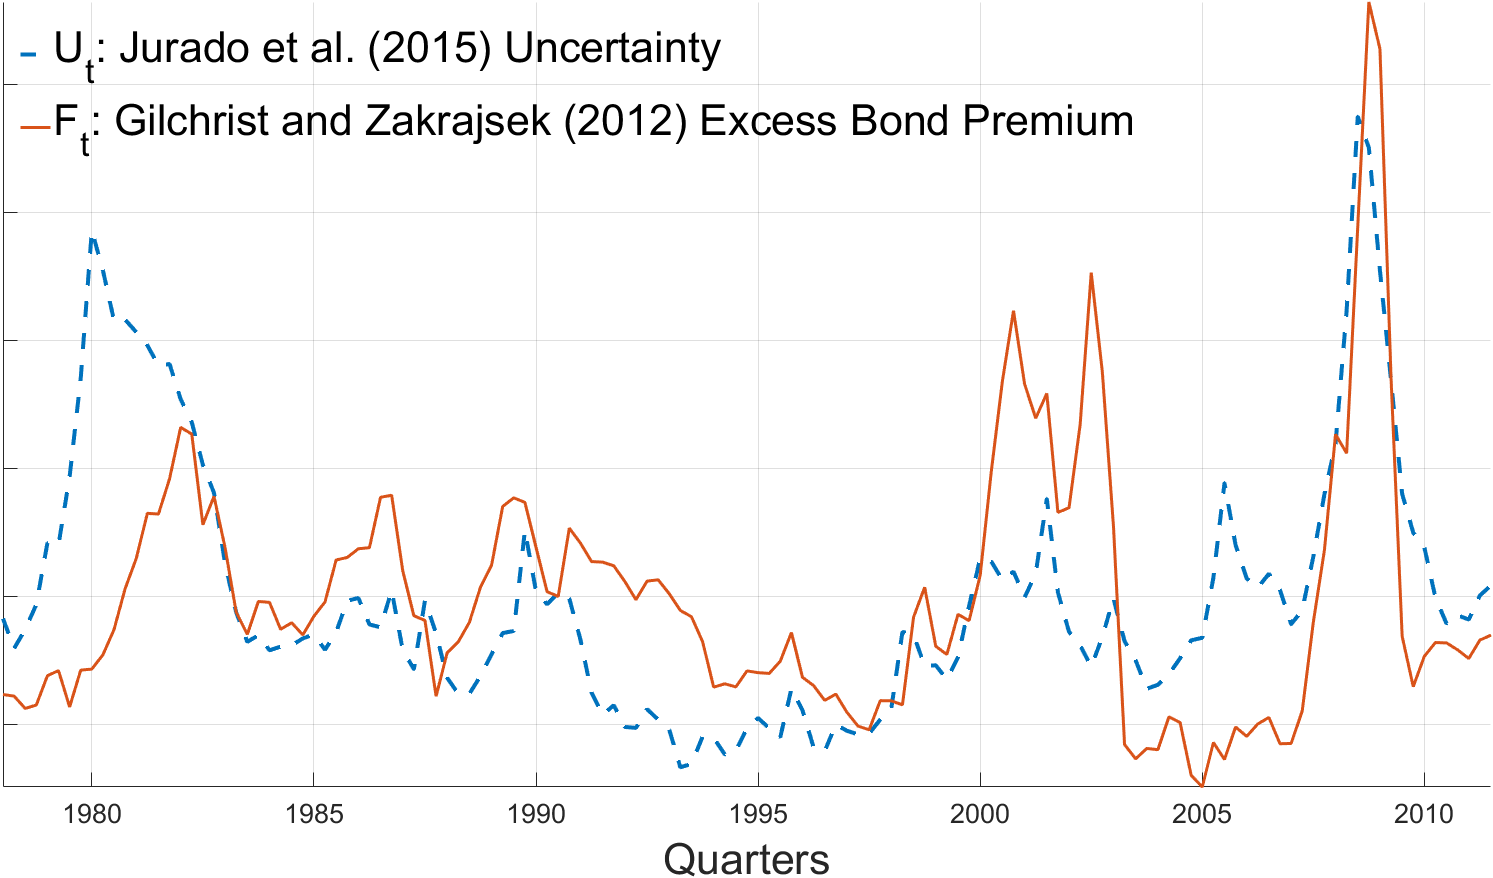
\includegraphics[scale=0.25]{Financial_Uncertainty}
			\label{fig:raw_data}
		\end{figure}
		
	}

	\frame{\frametitle{Motivation: Empirical Challenge in Structural VAR}	
	
	Empirically distinguishing between financial and uncertainty shocks is difficult
	\begin{itemize}
		\item[$\Rightarrow$] financial distress is empirically associated with larger volatility 
	\end{itemize}

\


Within a SVAR framework, this correlation significantly complicates identification of both shocks
\begin{enumerate}
	\item Implausible \textbf{zero-contemporaneous restrictions}
	\begin{itemize}
		\item[$\Rightarrow$] Both $F_t$ and $U_t$ are fast moving
	\end{itemize}	
	\item Unavailable instruments for \textbf{sign restrictions}	
	\begin{itemize}
		\item[$\Rightarrow$] Current theoretical models predict same qualitative effects on both prices and quantities
	\end{itemize}
\end{enumerate}
	
	
}





\frame{\frametitle{My contribution}
	
	I want to take a step back and show evidence and theory that financial and uncertainty shocks are \textbf{qualitative different}.
	
	
	\
		
	
	
	
	In particular, 
	
	
	\begin{enumerate}
		\item \textbf{Corporate cash holdings} respond differently to financial and uncertainty shocks. 
		\begin{itemize}
			\item[$\Rightarrow$] Identification assumption
			\end{itemize}
		
		\	
		
		\item I provide a \textbf{new econometric tool} to simultaneously identify two structural shocks when an internal instrument is available.\begin{itemize}
			\item[$\Rightarrow$] Generalized Penalty Function Approach  
		\end{itemize}
		
	\end{enumerate}
}

\frame{\frametitle{Roadmap}
	\Large{
		$ \ \ \ \ \ $ 1. \textbf{Cash Holdings}
		
		$ \ \ \ \ \ $ 2. Model
		
		$ \ \ \ \ \ $ 3. Empirical Strategy
		
		$ \ \ \ \ \ $ 4. Results
		
		$ \ \ \ \ \ $ 5. Conclusions
	}
}
	

\frame{\frametitle{Corporate Cash Holdings}
	
	\
	
\textbf{Cash and Cash Equivalents} refer to assets a business holds as ready cash
\begin{itemize}
	\item Coffer as petty cash
	\item Bank accounts
	\item Certificates of deposits
\end{itemize}

\

U.S. large firms have cash equal to about 15\% of total assets.

\

It is a \textbf{stock variable}, 
$$
Cash_t = Cash_{t-1} + NY_t + \delta K_t - I_t + B_t - D_t.
$$



}


\frame{\frametitle{Cross-Sectional Evidence}
	
	\textbf{Cash} and \textbf{Financial Frictions}
	\begin{itemize}
		\item[$\Rightarrow$] Cash is a substitute for external finance 
		\item[] \textit{Kaplan and Zingales (1997); Almeida, et al. (2004); Campello at al. (2010); Campello et al. (2011).}
	\end{itemize}

\

\textbf{Cash} and \textbf{Uncertainty}
	\begin{itemize}
	\item[$\Rightarrow$] Cash is positively associated with uncertainty shocks 
	\item[] \textit{Han and Qiu (2007); Baum et al. (2008); Bloom et al. (2018); Alfaro et al. (2018).}
\end{itemize}


}
		


\frame{\frametitle{Aggregate Evidence}

Aggregate quarterly cash (CHEQ) and assets (ATQ) using \textbf{Compustat} from 1961 to 2018.

\

Remove seasonality using 7-term Henderson filter on aggregate cash and aggregate assets and obtain \textbf{Cash2Assets}.

\


	\begin{table}[h!]
	\centering
	\begin{tabular}{llcc} \hline \hline
		                         & $\Delta$GDP         & U                &                   F    \\ 
		\hline
		\textit{Correlations}    &                     &                  &                                            \\ 
		U                        &      $-0.48^{***}$                &                  &                    \\
		F                        &  $-0.36^{***}$   &     $0.22^{***}$       &                             \\ 
		C2A                      &     $-0.06  $               &       $0.43^{***}$      &            $-0.37^{***}$           \\ 
		\hline \hline
	\end{tabular}
\end{table}



}

\frame{\frametitle{Roadmap}
	\Large{
		$ \ \ \ \ \ $ 1. Cash Holdings
		
		$ \ \ \ \ \ $ 2. \textbf{Model}
		
		$ \ \ \ \ \ $ 3. Empirical Strategy
		
		$ \ \ \ \ \ $ 4. Results
		
		$ \ \ \ \ \ $ 5. Conclusions
	}
}
	
	
%\frame{\frametitle{Economic Intuition I}	
		
%To provide an economic intuition of the differential response of \textbf{cash holdings} to uncertainty and financial shocks, I present a properly augmented model in the spirit of 
%\begin{itemize}
	%\item Almeida, Campello, and Weisbach (2004)
	%\item Han and Qiu (2007)
%\end{itemize}

%\

%It is a simple representation of a dynamic setting where a credit-constrained profit-maximizing firm has a trade-off between present and future investment opportunities
		
%}

\frame{\frametitle{Model - General Setup}

\begin{itemize}

\item \textbf{Three-period partial equilibrium} model

\	

\item Firm \textbf{maximizes} sum of \textbf{dividends} 
\begin{itemize}
\item Discount factor $\beta$ is one
\end{itemize}

\

\item \textbf{Choice variables} are
\begin{itemize}
	\item \textbf{Investments} $i_0$ and $i_1$ in period 0 and 1
	\item Amount to \textbf{borrow} $b_0$ and $b_1$ in period 0 and 1
	\item \textbf{Cash} $c$ in period 0 to be carried in period 1
\end{itemize}

\


\item Feature \textbf{financial frictions} in the form of risk premium

\

\item \textbf{Gross returns} $g(\cdot)$ happen in the last period for both investments
\begin{itemize}
	\item where $g'(\cdot) > 0$ and $g''(\cdot) < 0$.
\end{itemize}
	
	\end{itemize}





}

\frame{\frametitle{Model - Analytical Setup}
	
	

\begin{itemize}
	\item[]
\begin{itemize}
     \item[Period 0] $ \ \ \ d_0 = y_0 + b_0 - i_0 - c$
	
	\
	
	
	\item[Period 1] $ \ \ \ d_1 = y_1 + b_1 - i_1 + c, \ \ \ $ where $ \ y_1 \sim F(y_0,\sigma^2)$
	
	\
	
	
	\item[Period 2] $ \ \ \ d_2 = g(i_0) - b_0(1 + r_0) + g(i_1) - b_1(1 + r_1)$
\end{itemize}
\end{itemize}

\begin{eqnarray*}
	\begin{aligned}
\max_{\{ b_t,i_t,c \}_{t=0,1}} \ \ &\E \Big[  d_0 + d_1 + d_2     \Big| F  \Big] \\
\text{subject to} \ \ &r_0 = \frac{1}{2}\alpha_0 b_0 \ \ \text{and} \ \ r_1 = \frac{1}{2}\alpha_1 b_1 \\
&d_t \geq 0, \ \ \ t = 0,1,2 \\
\end{aligned}
\end{eqnarray*}

\

\begin{center}
Financial shock: $\uparrow \alpha_0$ $ \ \ \ \ $ vs $ \ \ \ \ $ Uncertainty shock: $\uparrow \sigma^2$
\end{center}
	
}


\frame{\frametitle{Solution}
	
	Assuming that firm needs external finance in equilibrium, model implies: 
\begin{itemize}
	\item $i_0 = y_0 + b_0 - c$,
	\item $i_1 = y_1 + b_1 + c$,
\end{itemize}
and first order conditions are
\begin{itemize}
	\item[$b_0:$] $g'(y_0 + b_0^* - c^*) = \underbrace{1 + \alpha_0 b_0^*}_{\text{Marginal Cost of $i_0$}}$
	
	
	\
	
	\item[$b_1:$] $\E \Big[ g'(y_1 + b_1^* + c^*) \Big] = \underbrace{1 + \alpha_1 b_1^*}_{\text{Marginal Cost of $i_1$}}$
	
	
	\
	
	
	\item[$c:$] $\underbrace{\E \Big[ g'(y_1 + b_1^* + c^*) \Big]}_{\text{Expected Marginal Return of $i_1$}} = \underbrace{g'(y_0 + b_0^* - c^*)}_{\text{Marginal Return of $i_0$}}$
\end{itemize}

}


%$\E_0 \Big[ g(y_t) \Big] > 1$ for $t=0,1$
%\begin{itemize}
	%\item[$\Rightarrow$] $d_t = 0 \ \ $ for $ \ t=0,1$
%\end{itemize}

%Objective function is,
%\begin{eqnarray*}
	%\begin{aligned}
	%	\max_{b_0,b_1,c} \ \ &g \big( i_0 \big) - b_0 - \frac{1}{2} \alpha_0 b_0^2 - y_0 + \E \bigg[  g \big( i_1 \big) - b_1 - \frac{1}{2} \alpha_1 b_1^2 - y_1   \bigg| F     \bigg]
	%\end{aligned}
%\end{eqnarray*}

\frame{\frametitle{Comparative Statics}
	
\begin{itemize}
	\item[$b_0:$] $g'(y_0 + b_0^* - c^*) = \underbrace{1 + \alpha_0 b_0^*}_{\text{Marginal Cost of $i_0$}}$
	
	
	\
	
	\item[$b_1:$] $\E \Big[ g'(y_1 + b_1^* + c^*) \Big] = \underbrace{1 + \alpha_1 b_1^*}_{\text{Marginal Cost of $i_1$}}$
	
	
	\
	
	
	\item[$c:$] $\underbrace{\E \Big[ g'(y_1 + b_1^* + c^*) \Big]}_{\text{Expected Marginal Return of $i_1$}} = \underbrace{g'(y_0 + b_0^* - c^*)}_{\text{Marginal Return of $i_0$}}$
\end{itemize}

\
	
\textbf{Uncertainty shock}: $y_1 \sim Q$ which is mean-preserving spread in $F$
	\begin{enumerate}
	\item[$\Rightarrow$] $c^*(\alpha_0,Q) > c^*(\alpha_0,F)$ as long as $g'''(\cdot) > 0$
\end{enumerate}

\

\textbf{Financial shock}: $\alpha_0^f > \alpha_0$ which is an exogenous increase in $r_0$
	\begin{enumerate}
	\item[$\Rightarrow$] $c^*(\alpha_0^f,F) < c^*(\alpha_0,F)$ 
\end{enumerate}



}



\frame{\frametitle{Roadmap}
	\Large{
		$ \ \ \ \ \ $ 1. Cash Reserves
		
		$ \ \ \ \ \ $ 2. Model
		
		$ \ \ \ \ \ $ 3. \textbf{Empirical Strategy}
		
		$ \ \ \ \ \ $ 4. Results
		
		$ \ \ \ \ \ $ 5. Conclusions
	}
}












\frame{\frametitle{Empirical Analysis}
	
	

Given the reduced-form system $X_t = B(L) X_{t-1} + \iota_t$ where

$$
X_t = \begin{bmatrix}
U_t \\
F_t \\
GDP_t \\
C_t \\
I_t \\
H_t \\
C2A_t \\
GDPDef_t \\
\end{bmatrix}
$$ 

\

Dataset ranges from 1978q1 to 2015q3.


	
}

\frame{\frametitle{Objective of the Empirical Strategy}

Given the reduced-form system $X_t = B(L) X_{t-1} + \iota_t$, 

$\Rightarrow$ find a rotation of $\Sigma_{\iota} = \iota_t' \iota_t$ such that

\begin{enumerate}
	\item it allows $F_t$ and $U_t$ to respond to both shocks on \textbf{impact}
	\item it respects \textbf{sign-restriction} assumptions on cash
	\item it is \textbf{unique}
	\item it delivers shocks \textbf{orthogonal} to each other
	\item it is unaffected by the \textbf{order} of the estimation
\end{enumerate}


}





\frame{\frametitle{Sequential Penalty Function Approach ($\delta \geq 0$)} 
	
	\
	
	\textbf{1. Uncertainty Shock}
	\begin{eqnarray*}
		\begin{aligned}
		\max_{\gamma_{U}} \ \ \ \ \ &  \ \underbrace{e_U A_0 \gamma_U}_{\text{Impact on U}} \ \ \  + \ \ \ \textcolor{red}{\delta} \underbrace{e_{C} A_0 \gamma_U}_{\text{Impact on Cash}} \\
		\end{aligned}
	\end{eqnarray*}

\textbf{Intuition}. $\gamma_{U}$ increases both uncertainty and cash on impact.

\

	\textbf{2. Financial Shock}
	\begin{eqnarray*}
		\begin{aligned}
		\max_{\gamma_{F}} \ \ \ \ \ & \  \underbrace{e_F A_0 \gamma_F}_{\text{Impact on F}} \ \ \  - \ \ \  \textcolor{red}{\delta} \underbrace{e_{C} A_0 \gamma_F}_{\text{Impact on Cash}} \ \ s.t. \ \ \underbrace{\textcolor{red}{\gamma_U \gamma_F' = 0}}_{\text{Orthogonality with U shock}} \\
		\end{aligned}
	\end{eqnarray*}

\textbf{Intuition}. $\gamma_{F}$ increases uncertainty and decreases cash on impact.
	
}

\frame{\frametitle{Sequential Penalty Function Approach ($\delta \geq 0$)} 
	
		\
	
	\textbf{1. Financial Shock}
	\begin{eqnarray*}
		\begin{aligned}
			\max_{\gamma_{F}} \ \ \ \ \ & \  \underbrace{e_F A_0 \gamma_F}_{\text{Impact on F}} \ \ \  - \ \ \  \textcolor{red}{\delta} \underbrace{e_{C} A_0 \gamma_F}_{\text{Impact on Cash}}  \\
		\end{aligned}
	\end{eqnarray*}
	
	\textbf{Intuition}. $\gamma_{F}$ increases uncertainty and decreases cash on impact.
	
	\
	
	\textbf{2. Uncertainty Shock}
	\begin{eqnarray*}
		\begin{aligned}
			\max_{\gamma_{U}} \ \ \ \ \ &  \ \underbrace{e_U A_0 \gamma_U}_{\text{Impact on U}} \ \ \  + \ \ \ \textcolor{red}{\delta} \underbrace{e_{C} A_0 \gamma_U}_{\text{Impact on Cash}} \ \ s.t. \ \ \underbrace{\textcolor{red}{\gamma_U \gamma_F' = 0}}_{\text{Orthogonality with F shock}} \\
		\end{aligned}
	\end{eqnarray*}
	
	\textbf{Intuition}. $\gamma_{U}$ increases both uncertainty and cash on impact.
	
}

\frame{\frametitle{Generalized Penalty Function Approach} 

	\
	
	\textbf{1. Financial Shock}
	\begin{eqnarray*}
		\begin{aligned}
			\max_{\gamma_{F}} \ \ \ \ \ & \  \underbrace{e_F A_0 \gamma_F}_{\text{Impact on F}} \ \ \  - \ \ \  \textcolor{red}{\delta^*} \underbrace{e_{C} A_0 \gamma_F}_{\text{Impact on Cash}}  \\
		\end{aligned}
	\end{eqnarray*}
	
	
	\textbf{2. Uncertainty Shock}
	\begin{eqnarray*}
		\begin{aligned}
			\max_{\gamma_{U}} \ \ \ \ \ &  \ \underbrace{e_U A_0 \gamma_U}_{\text{Impact on U}} \ \ \  + \ \ \ \textcolor{red}{\delta^*} \underbrace{e_{C} A_0 \gamma_U}_{\text{Impact on Cash}}  \\
		\end{aligned}
	\end{eqnarray*}

where $\textcolor{red}{\delta^*}$ is chosen such that $\textcolor{red}{\gamma_U \gamma_F' = 0}$.

\	 

\textbf{Economic Intuition.} Weight of sign restrictions should be large enough such that the two shocks are separated without any external constraint.

}


%	\text{subject to} \ \ \ \ \  & \ \delta \geq 0 \ \ \ \ \ \ \text{and} \ \ \ \ \ \  \underbrace{\gamma_U \gamma_U' = 1}_{\text{Normalization}}

%		\text{subject to} \ \ \ \ \ \ & \ \delta \geq 0, \ \ \ \ \ \ \ \underbrace{\gamma_F \gamma_F' = 1}_{\text{Normalization}}, \ \ \ \ \ \ \text{and} 



\frame{\frametitle{Roadmap}
	\Large{
		$ \ \ \ \ \ $ 1. Cash Reserves
		
		$ \ \ \ \ \ $ 2. Model
		
		$ \ \ \ \ \ $ 3. Empirical Strategy
		
		$ \ \ \ \ \ $ 4. \textbf{Results}
		
		$ \ \ \ \ \ $ 5. Conclusions
	}
}

\frame{\frametitle{Uncertainty Shock}

\begin{center}
	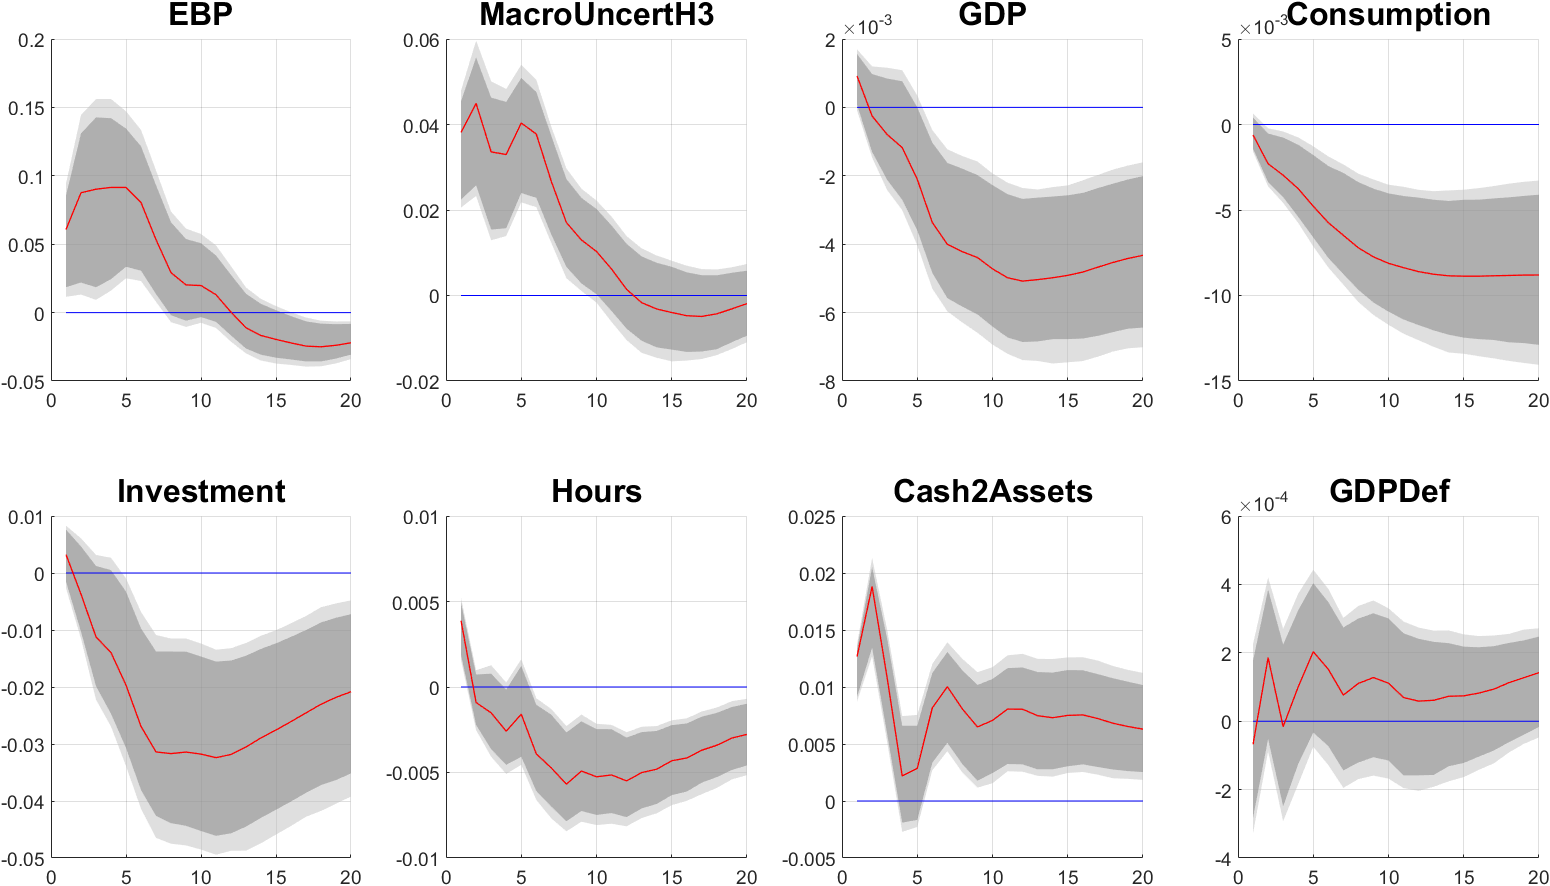
\includegraphics[scale=0.27]{fig_Uncertainty_Shock_GPFA_Compustat_3lags_gamgamZero}
\end{center}	

	
}

\frame{\frametitle{Financial Shock}
	
	\begin{center}
		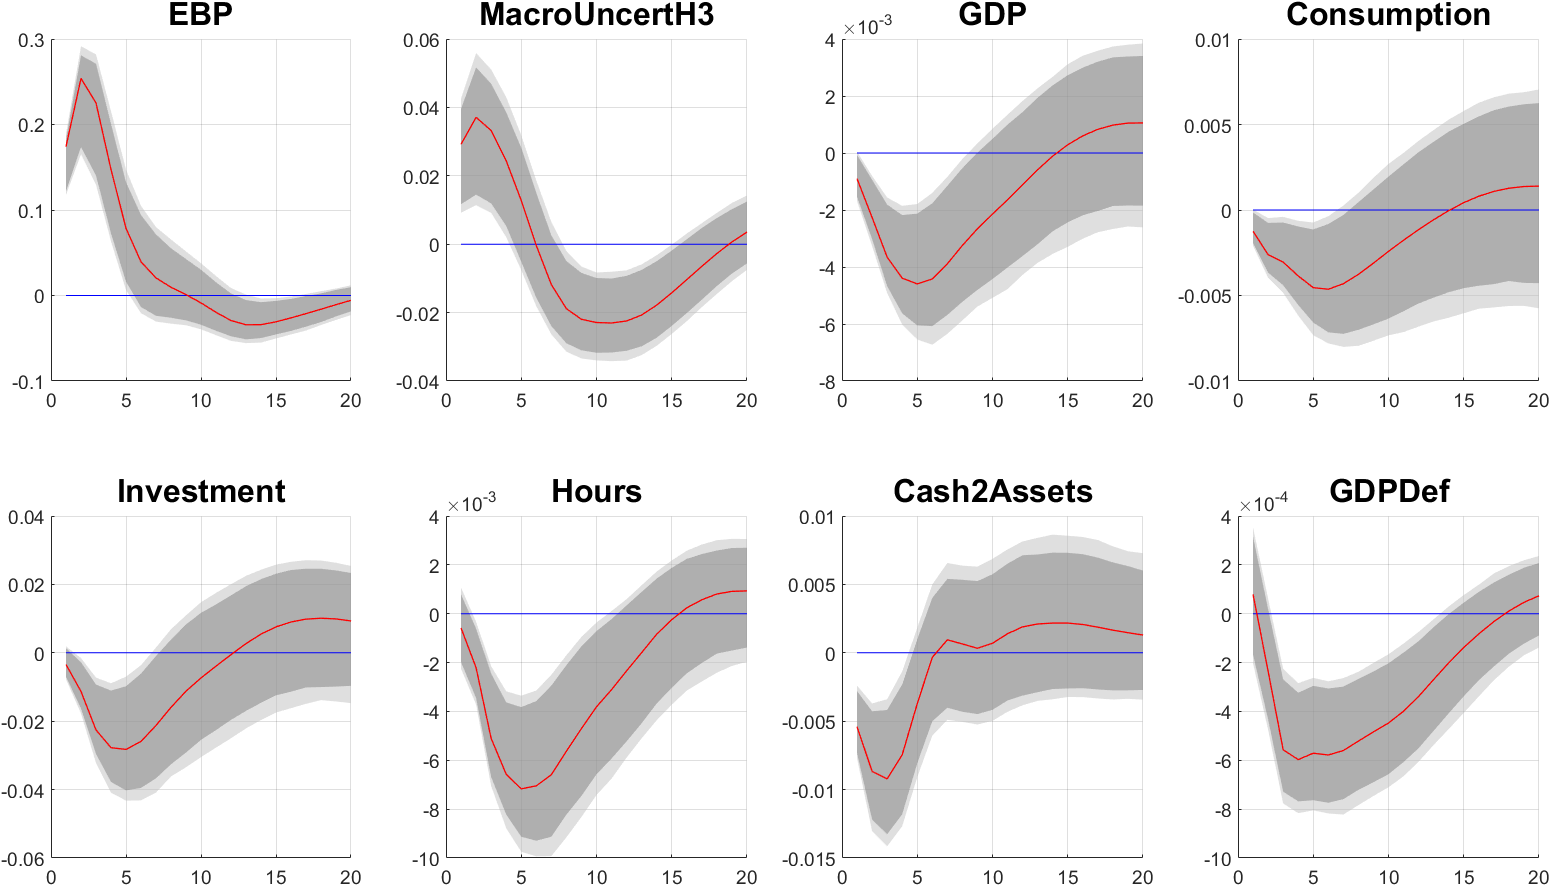
\includegraphics[scale=0.27]{fig_Financial_Shock_GPFA_Compustat_3lags_gamgamZero}
	\end{center}	
		
}



\frame{\frametitle{Variance Explained}
	
	\begin{center}
		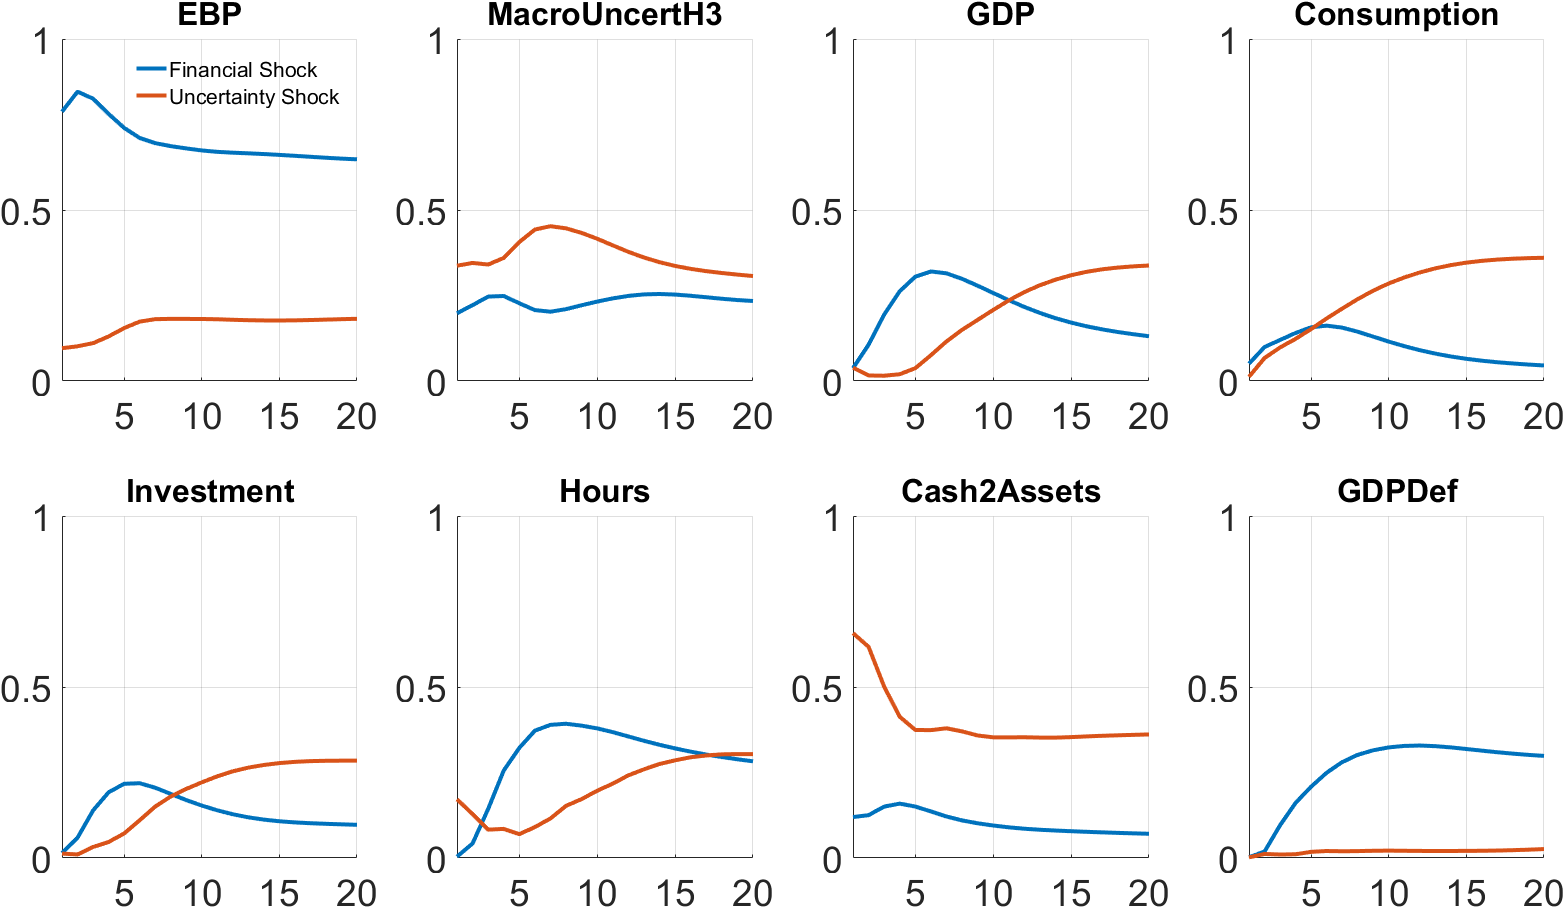
\includegraphics[scale=0.27]{fig_var_dec_vardec_GPFA_Compustat_3lags_gamgamZero}
	\end{center}	
	
}

\frame{\frametitle{Roadmap}
	\Large{
		$ \ \ \ \ \ $ 1. Cash Reserves
		
		$ \ \ \ \ \ $ 2. Model
		
		$ \ \ \ \ \ $ 3. Empirical Strategy
		
		$ \ \ \ \ \ $ 4. Results
		
		$ \ \ \ \ \ $ 5. \textbf{Conclusions}
	}
}

\frame{\frametitle{Conclusions}
	
	

	


\begin{itemize}
	
	

\item \textbf{Cash reserves} as an internal instrument to simultaneously identify financial and uncertainty shocks.

\

\item An \textbf{econometric tool} to overcome known SVAR shortcomings
\begin{itemize}
	\item[$\Rightarrow$] Tests using simulated data confirm the reliability of the procedure. See \textbf{Appendix A}.
\end{itemize}

\


\item Empirical results confirm the \textbf{relevance} and \textbf{exogeneity} of both shocks.
\begin{itemize}
	\item[$\Rightarrow$] Correlations with external shocks is available in \textbf{Appendix B}.
\end{itemize}

\


\item \textbf{Financial shocks} have larger effects in the \textbf{short run} while \textbf{uncertainty shocks} have a more \textbf{persistent} effect.

\end{itemize}


}

\frame{\frametitle{Next Steps}
	
	\begin{enumerate}

\item Empirical evidence in favor of my identification assumption

\begin{itemize}
	\item Using \textbf{Quarterly Financial Report} data to show that my results are mostly driven by small firms 
	\item Merging \textbf{Compustat} and \textbf{TRACE} to show firm-level evidence of the differential response of cash
	$$
	\frac{Cash_{it}}{Assets_{it}} = \underbrace{\beta^U}_{(+)} U_{it} + \underbrace{\beta^F}_{(-)} F_{it} + \beta^X X_{it} + \delta_i + \lambda_t + \varepsilon_{it}
	$$
\end{itemize}


\


\item Design and analyze a \textbf{dynamic GE model} 
\begin{itemize}
	
	\item to show my identification assumption survives to GE effects
	
	\item to test whether GPFA can recover both shocks
	
\end{itemize}


\end{enumerate}

}

\frame{\frametitle{Appendix A - Simulated Data and Generalized PFA}
	
	Consider the following structural model,
	
	\begin{itemize}
		\item $U_t = B_{UU} U_{t-1} + B_{UF} F_{t-1}  + B_{UC} C_{t-1}  +  A_{UU}s_t^U  +  A_{UF}s_t^F$
		\item $F_t = B_{FU} U_{t-1} + B_{FF} F_{t-1}  + B_{FC} C_{t-1}  +  A_{FU}s_t^U  +  A_{FF}s_t^F$
		\item $C_t = B_{CU} U_{t-1} - B_{CF} F_{t-1}  + B_{CC} C_{t-1}  +  A_{CU}s_t^U  -  A_{CF}s_t^F$
		\end{itemize}
where $s_t^U \sim N(0, \sigma^2_U)$, $s_t^F \sim N(0, \sigma^2_F)$ and $s_t^U \perp s_t^F$.

\
	
	Objective is to estimate structural parameters 
	\begin{itemize}
		\item using only $X_t = [U_t, \ F_t, \ C_t]$, and
		\item only knowing that $A_{ji} \geq 0$ for $j,i = \{U, \ F, \ C \}$.
	\end{itemize} 
	$\Rightarrow$ apply GPFA to test reliability of the econometric tool
}


\frame{\frametitle{Appendix A - Small Sample Performance (T = 100)}
	
\begin{center}
	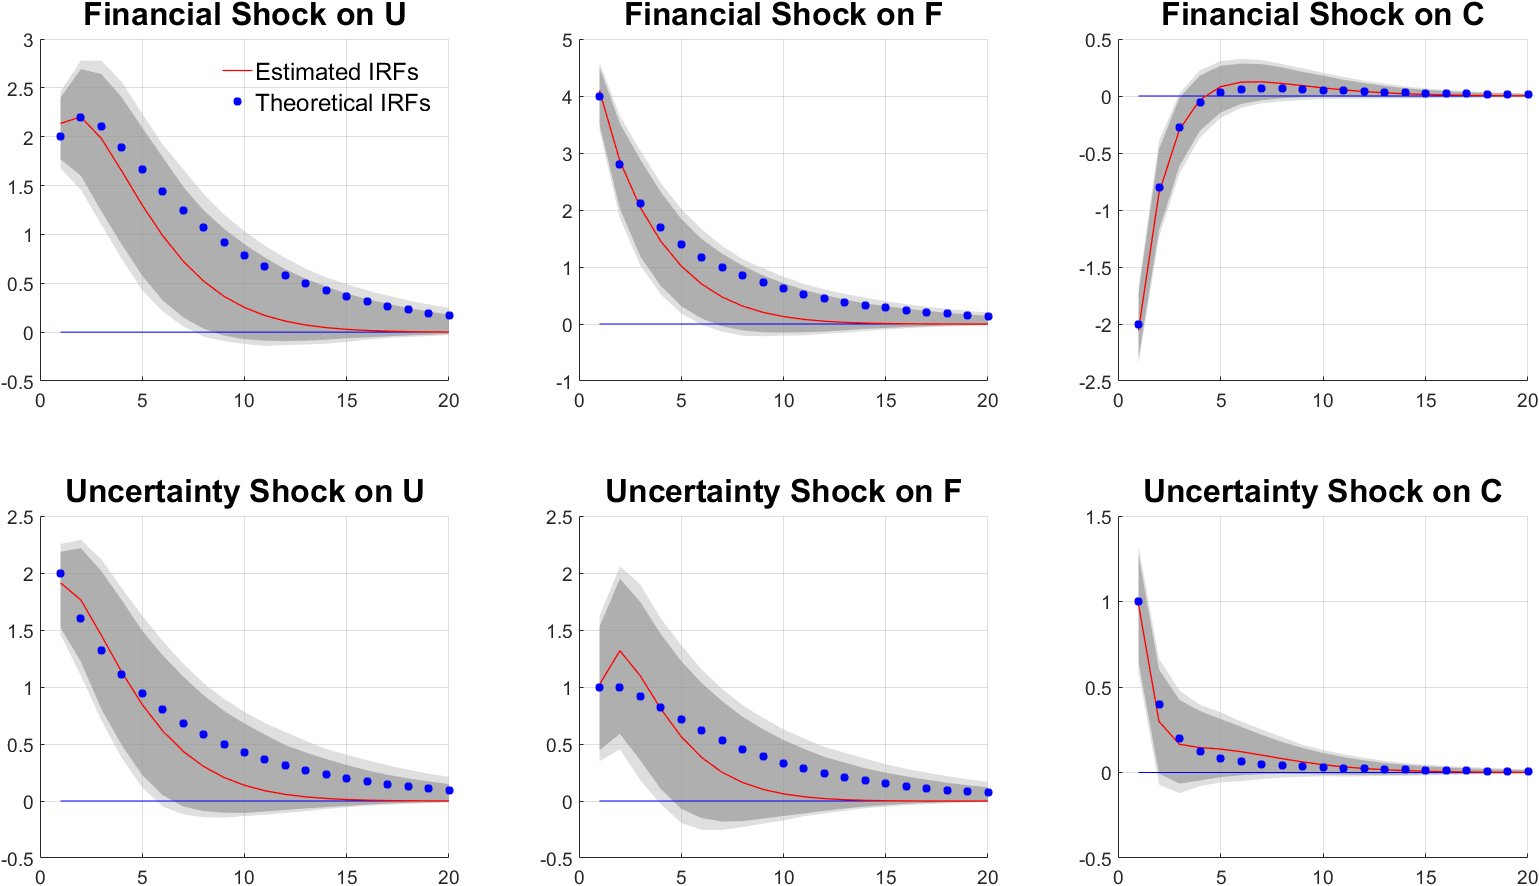
\includegraphics[scale=0.27]{test_small}
\end{center}	

	
}



\frame{\frametitle{Appendix A - Large Sample Performance (T = 100000)}
	
\begin{center}
	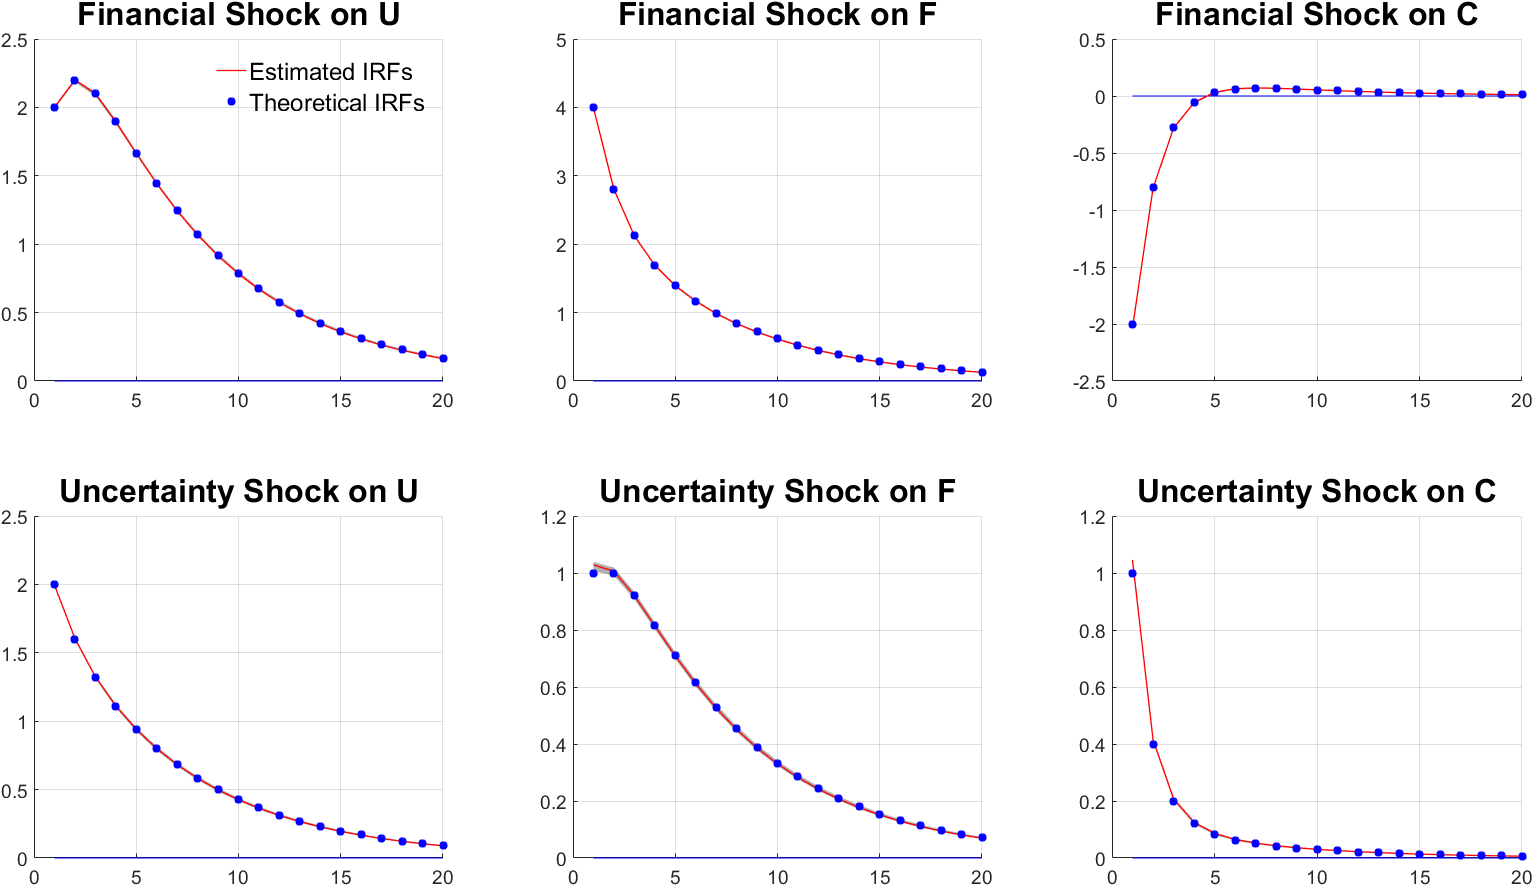
\includegraphics[scale=0.27]{test_large}
\end{center}		
	
}


\frame{\frametitle{Appendix B - Correlations with Other External Shocks}
	
	
	\begin{table}[h!]
		\centering
		\begin{tabular}{lrr} \hline \hline
			                & \textbf{Uncertainty Shocks} & \textbf{Financial Shocks} \\ 
			                \hline
			\textit{External Shocks} &                    &                      \\ 
			BZP Military News        & $-0.10$  $(0.24)$  &   $0.08$  $(0.31)$   \\ 
			Ramey Military news      &  $0.07$  $(0.44)$  &   $0.02$  $(0.82)$   \\ 
			LWY Exp. Tax             &  $0.03$  $(0.74)$  &   $0.15$  $(0.11)$   \\ 
			RRMR Unexp. Tax          & $-0.13$  $(0.16)$  &   $0.05$  $(0.59)$   \\ 
		    RRMR Exp. Tax            & $-0.08$  $(0.36)$  &   $0.03$  $(0.76)$   \\ 
		    AdjTFP AR(1)             &  $0.08$  $(0.31)$  &  $-0.14$  $(0.11)$   \\ 
		    RR Mon. Policy           & $-0.13$  $(0.18)$  &  $-0.04$  $(0.70)$   \\ 
		    \hline \hline
		\end{tabular}
	\end{table}
		
	
}













\end{document}